\section{Background}
\label{BabyGotBack}
GPGPU (General-purpose computing on graphics processing units) has been on the rise, due to limitation for CPU's, such as power limitation, and the fact that the computational potential of GPU's (Graphical processing unit) is vastly greater than CPU's, see Figure \ref{potential}. There are technical/physical issue in reaching this potential, for example memory bandwidth, but there is also the conceptual issue of how to map parallelism to parallel hardware.
\begin{figure}[h]
\centering
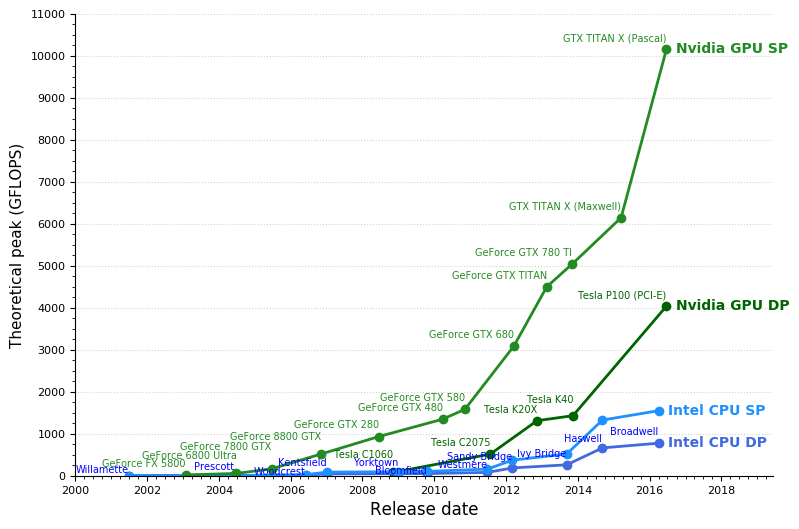
\includegraphics[width=.8\textwidth]{resources/graf.png}
\caption{A graph showing the computational potential of CPUs and GPUs from 2000---2016 \cite{cpu-vs-gpu}}
\label{potential}
\end{figure}
\begin{comment}
A common way to increase computer performance, is to increase the capacity for parallelism. For practical usage, however, this is difficult to implement, due to low-level GPU-specific languages requiring domain specific knowledge to make full use of that capacity. A vast amount of work has gone into transforming high-level hardware-agnostic code into these low-level GPU-specific languages \cite{inc-flat}. 
\end{comment}

\subsection{Parallelism} 
% HVORDAN VI FORMULERE LIMITATION
In the real world we have limitations to our current parallel hardware. We commonly execute parallel work on GPU's, due to its high number of threads. The limitation on GPU's, most essential to this report, is that a thread, may not spawn additional threads (this is not strictly true, but in practice it remains so). Therefore we need to work within that limitation. We say that since a GPU thread cannot spawn additional threads, it only supports \textit{flat} parallelism. In the following sections we will look at approaches to work within this limitation.    

\subsection{Flat parallelism}
Many problems does not have a flat structure, as our current platform effectively requires. Imagine a function (\texttt{drawline}) that, given two endpoints, will determine all the pixel that lie in a straight line in between. This can be done in parallel, but since only flat, and not nested parallelism is supported, we cannot call \texttt{drawline} within another parallel function (for example a \texttt{drawObject} function) \cite{flat}. 

Therefore we need to map nested parallelism to a flat structure. This problem has already been conceptually solved by \textit{flattening}, and implemented in the language NESL \cite{nesl}. The basic idea is to flatten the nested data that is to be worked on, and performing operations on that data in parallel. 

When flattening a datastructure, we want to keep the information regarding the nest. In the original work, presenting flattening \cite{flat}, this is done with a structure called \textit{field} which has the form of \texttt{(nest information, value)}, where a value can be an additional field, allowing for arbitrary depth. For a multidimensional array the field would be \texttt{(length, vaule/field)}, below here is a concrete example.
\begin{center}
\texttt{[[1,2,3],[4,5],[6,7,8,9]] $\to$ ([3], ([3,2,4], [1,2,3,4,5,6,7,8,9]))}
\end{center}
This allows for a completely flat array, that can be mapped directly to the GPU. However the concept of flattening has practical issues. GPU's are not infinitely parallel, it has some capacity for parallelism,< and going beyond that will result in more overhead, than computational gain. This problem is in no way addressed by flattening. Along with overhead, comes the issue that parallelism effectively destroys information about access patterns, making locality optimizations pretty much impossible, so we end up with greater overhead than gain, along with losing potential optimizations, when we always use the maximum parallelism available (fully flatten datastructures). 

\subsection{Futhark}
The problem of mapping parallelism to flat hardware, and the difficulty of writing parallel code, in GPGPU languages such as CUDA and OpenCL, is what the programming language \textbf{Futhark} aims to solve. The creator of Futhark writes the purpose, of the language, nicely on the home page for the language \textit{"Because it’s nicer than writing CUDA or OpenCL by hand!"} \cite{futhark-home}. On the same page, Futhark is described, more precisely, as \textit{"a statically typed, data-parallel, and purely functional array language"}, but better than a description, is an example:
\begin{center}
\lstset{language=haskell}
\begin{lstlisting}
let dotprod [n] (xs: [n]f32) (ys: [n]f32): f32 =
	reduce (+) 0f32 (map2 (*) xs ys)

let main [n][m][p] (xss: [n][m]f32) (yss: [m][p]f32): [n][p]f32 =
	map (\xs -> map (dotprod xs) (transpose yss)) xss
\end{lstlisting}%
\captionof{lstlisting}{Matrix-matrix multiplication in Futhark \cite{ppopp}}
\label{matmultFuthark}
\end{center}
A Futhark program for matrix-matrix multiplication can be seen in listing \ref{matmultFuthark}, the syntax is similar to languages such as ML, and Haskell. It is a good example of how Futhark differs from CUDA or OpenCL (we would have liked to include an example of CUDA, but it was to long, so see \ref{cuda-matmult} for that). It allows the programmer to write efficient parallel code, without all the hardware specific knowledge regarding massively parallel systems. 

The reason for Futhark being a functional language, is that functional languages lends themselves well to parallel problems, due to the functional paradigm not relying on evaluation order and side effects, as much as other many other paradigms. An example of this is \texttt{map}, which can process each element in parallel. However along with the problem of flat parallelism being required by the hardware, among other issues like to small of a stack and no function pointers, a functional language by itself is not a solution, and modifying an existing language such as Haskell is not optimal due to the size and expressiveness of it, being poorly suited for the restrictive nature of a GPU's. 

In the following sections we will look at how Futhark solves the problem of
GPU's requiring flat parallelism, and the solution even being independent from
this limitation. An example of a simple problem, that is not flat, is the
\texttt{dotprod} function from listing \ref{matmultFuthark}. Here there is a \texttt{map2}\footnote{\texttt{map2} is a variant of \texttt{map} taking two arrays instead of a single element and an array. For example \texttt{map2 (+) [1,2,3] [4,5,6] $\to$ [5,7,9]}} which is nested inside of a \texttt{reduce}\footnote{Reduce does not obviously appear to be a parallel construct, due to the elements being dependent on each other, however this is done by a \textit{segmented reduce} \cite{segred}, making it effectively so.}, both operations are parallel, thereby giving \textit{nested parallelism}. In more general terms, nested parallelism is when there are parallel constructs nested within each other. Futhark supports such nested parallelism. More specifically, Futhark supports nested \textit{data}-parallelism. Data-parallelism is when some function/operation, is applied to a dataset in parallel, such that one thread uses function \texttt{x} on a subset of data \texttt{y}, and another thread also uses function \texttt{x}, but on a different subset of \texttt{y}. Other languages/environments that support nested data-parallelism are the likes of; CUDA, Open MP, OpenCL, NESL etc. With NESL being the conceptual precursor to the other languages. As mentoned earlier, NESL solved the issue of nested data-parallelism by flattening data structures (both regular and irregular), resulting in maximum parallelism, which can be inefficient. Therefore we need to determine when it is useful to exploit more parallelism. 

\subsection{Moderate flattening}
To determine the amount of parallelism to exploit, we need a closer loke at GPU's. In the world of GPU's we have \textit{kernel}s, and a kernel is simply a GPU program. In CUDA specifically, it allows the programmer to define a function, that, when called, is executed \textit{N} times in parallel by \textit{N} different \textit{CUDA threads} or \textit{CUDA blocks}\footnote{For a further explanation of threads and blocks see \cite[p. 5-9]{prog-guide-cuda}}. Such a function is called a kernel, and an example of a CUDA kernel is the matrix-matrix multiplication in appendix \ref{cuda-matmult}. 

A kernel can be thought of as the work, that is to be done, in a perfect \textit{parallel nest}. A perfect parallel nest is a nest where all the work, is at the innermost level. 
\begin{figure}[h]
\centering
	\subfloat[][Code fragment before distribution.]
	{
	\centering
	\begin{lstlisting}
map (\xs -> let y = reduce (+) 0 xs 
		in map (+y) xs)
	xss
\end{lstlisting}	
	\label{beforeDist} 
	}\hspace{2cm}
	\subfloat[][Code fragment after distribution.]
	{
	\centering
	\begin{lstlisting}
let ys = map (\xs -> reduce (+) 0 xs) xss
in map (\xs y -> map (+y) xs) xss ys
\end{lstlisting}
	\label{afterDist}
	}
	\caption{Two version of a fragment of code, showing the distribution of SOACs (\textit{second-order array combinators}) \cite{futhark-moderate-blog}.}
	\label{loopDist}
\end{figure}
\noindent Futhark transforms nested data-parallelism into structures, from
which kernels can later be extracted, and an example of this transformation can
be seen in figure \ref{loopDist}. We can see that the outer \texttt{map}, of
figure \ref{beforeDist}, contains more parallelism in it, in terms of the
parallel constructs \texttt{reduce} and \texttt{map}, so in the case where the
outer \texttt{map} does not saturate the GPU's capacity, we would want to
exploit the parallelism of the \texttt{map} body. With figure \ref{beforeDist}
this is not possible, since the outer \texttt{map} would be parallelised, and
the inner sequentialized to one GPU kernel. Instead we can transform it to
figure \ref{afterDist}. Here the SOACs of the body (the parallel constructs
\texttt{map} and \texttt{reduce}) in figure \ref{beforeDist}, are distributed out into their own \texttt{map} nests, giving two perfect \texttt{map} nests, and thereby translates to two GPU kernels, where the code of line 1 (eventual first kernel), is passed into the code of line 2 (eventual second kernel), allowing for further exploitation of the nested parallelism.

This transformation is dubbed \textit{moderate flattening} \cite{futhark-nested-para}, due to its conceptual resemblance to the flattening algorithm put forth by \citeauthor{flat} \cite{flat}. However it is moderate in its approach, due to it flattening the parallel construct until the parallelism saturates the hardware, after which it efficiently sequentialize the remaining parallelism. As we saw in Figure \ref{loopDist}, Futhark flattens nested parallel construct by extracting kernels, based on rewrite/flattening rules. At the time of implementing moderate flattening, the algorithm used to apply these rules where based on heuristics about the structure of \texttt{map} nest contexts. These where decent approximations but due to the nature of GPU's (having different capacities for parallelism) there is no one size fits all. 

It is important to note that Futhark does not currently support irregular data structures. This means that we cannot have a multidimensional array, where the elements have different shapes. The reason for this, is that to quantify an amount of parallelism, executed on a core efficiently, Futhark needs it to be regular. Irregular structures could be suspect to dynamic dependencies, and require more overhead because of the irregular memory access.  

\subsection{Incremental flattening}
While moderate flattening was a good start it lacks the ability to dynamically flatten appropriately to the hardware capabilities, and the size of the data being worked on. This is where incremental flattening comes in. In short incremental flattening statically generates multiple different, semantically equivalent, piecewise code versions of the same program, based on the rules of moderate flattening (along with some additional ones) \cite{inc-flat}, and then dynamically chooses whether or not to further exploit parallelism or not.  

To get an intuition for incremental flattening, lets go back to the matrix-matrix multiplication example in listing \ref{matmultFuthark}. Due to matrix-matrix multiplication containing a lot of \texttt{map}s (as many GPU programs do), we will briefly explain the code versions generated by the flattening rule, when a \texttt{map} containing additional parallelism, is encountered (CV is short for code version); 
\begin{itemize}
\item[CV0] The body of the map will be executed sequentially. This means that there will be assigned one GPU thread to each element of the array being mapped over, each thread executing the map body sequentially.
\item[CV1] The body of the map is partially executed in parallel. This means that there will be assigned one GPU group/block to each element of the array being mapped over. This is partial since it does not exploit the parallelism fully, due to, most likely, not having enough threads to fully parallelise the entire construct within the \texttt{map} body.
\item[CV2] Continues to flatten the \texttt{map} function, since we still have further parallel capacity to exploit.  
\end{itemize}
\begin{center}
	\centering 
	\begin{forest}
[\texttt{map}
	[CV0,edge]
	[additional parallelism,edge
		[CV1,edge]
		[CV2,edge]	
	]
]
\end{forest}
	\captionof{figure}{A tree showing the structure of the three different code versions generate by flattening a \texttt{map} nest}
	\label{maptree}
\end{center}
In matrix-matrix multiplication, there are three levels of nested parallelism to exploit; the outer and inner \texttt{map} on line 5, and the \texttt{dotprod} function. Lets look at the different ways we can execute the function, there are at least 5 different ways to execute the code, generating 5 different code versions (denoted by a V) \cite{inc-flat};
\begin{itemize}
	\item[V0)] The outer \texttt{map} is distributed out across the parallel construct, executing the body of the function sequentially. More specifically one GPU thread calculates one row in the resulting matrix each. This is CV0 for \texttt{map}.
	\item[V1)] The outer \texttt{map} is executed in parallel, and the inner \texttt{map} of \texttt{main} is executed partially in parallel. More specifically one GPU group/block calculates one row in the resulting matrix. This is CV1 for \texttt{map}. 
	\item[V2)] The two outer maps of \texttt{main}, are extracted as kernels and the kernel of the outer \texttt{map} will invoke the inner \texttt{map} kernel saturating the GPU, and the body of the two \texttt{map}s (\texttt{dotprod}) is executed sequentially. More specifically each GPU thread is calculating one element in the resulting matrix. This is CV0 for \texttt{map}.
	\item[V3)] The two outer \texttt{maps}, does not saturate the GPU, but the \texttt{dotprod} function would oversaturate it, therefore, \texttt{dotprod} is partially executed in parallel. More specifically each element of the result matrix is executed by a GPU group/block. This is CV1
	\item[V4)] If the entire parallel nest does not oversaturate the GPU, the entire nest is executed in parallel. This is CV2
\end{itemize} 
We have to choose between these different, but semantically equivalent, ways of execution. The optimal choice will depend on the hardware, and the data being worked on. To visualize the choices, we will look at them as a tree. In Figure \ref{MatMultTree} there are four choices, we have to consider, and these choices are dependent on each other
\begin{center}
	\centering 
	\begin{forest}
[Choice0
	[V0,edge ]
	[Choice1,edge 
		[V1,edge ]
		[Choice2,edge 
			[V2,edge ]
			[Choice3,edge 
				[V3,edge ]
				[V4,edge ]
			]
		]	
	]
]
\end{forest}
	\captionof{figure}{The structure of choices found in the futhark program for matrix-matrix multiplication (see listing \ref{matmultFuthark}). (V) represents the resulting code version of a choice}
	\label{MatMultTree}
\end{center}
With these dependent choices, the idea of incremental flattening becomes increasingly clear. We step through the code, and decided whether we should flatten the parallelism available (for example a \texttt{map} nest), or whether we should sequentialize it, and exploit locality-of-reference optimizations. Due to the dependency of the choices, we end up iterating through the parallel nest, and flattening until we reach the full capacity of the hardware, hence the name \textit{incremental flattening}. The choices will not always be in form of a unbalanced tree (although they are for the most part), they can also be balanced, and/or form a forest, we will give an example of a are more complicated tree later.

\subsection{Structure of the code versions}
%Bad section name
To further understand how we will choose the correct code version, we have filled out the matrix-matrix multiplication tree, with more detail, which can be seen in Figure \ref{MatMultTreeFilled}. In the tree, at the parent nodes, we see the statically generated predicates (the choice), hence forth known as \textit{threshold comparisons}, or just \textit{comparisons}, which guard the different code versions. The comparisons, have a \textit{threshold parameter} on the left $t_i$, which is a symbolic representation of the parallel capacity of the hardware. On the right of the comparison, we have a value, based upon the dataset given, and as seen in the figure, these will reflect the shape and size of the data.
\begin{comment}
The process of autotuning a Futhark program is, to automatically pick the fastest combination (or single) code versions, based on the hardware the program is executed on, and some representative data. In the process of selecting the appropriate code version we have three important terms we, that we be central to this report, and therefore we wish to clearly define them in the context of this report;	
\paragraph{Threshold parameter} or just \textit{threshold} is a value that symbolizes the capacity for parallelism (memory, thread count etc.), of the hardware the program is executed on.
\paragraph{Dataset value} is a value that represent some of the dataset given. For example for the outer \texttt{map} in matrix-matrix multiplication, the dataset value would (primarily) be constructed by the number of rows.
\paragraph{Predicate} threshold comparison, or just comparison, is a comparison between a threshold and a dataset value that guard which code version to use. \\
To pick the best version, we need to tune the threshold parameters, to values that will result en the combination of code versions that gives the fastest runtime. This process is called tuning. The guarding predicates are of the form $threshod \; \leq \; dataset\; value$. By default the threshold parameter is set to a value off $2^{15}$, as an estimate, but is likely sub-optimal. With these terms, we can now fill out the example in Figure \ref{MatMultTree}, getting Figure \ref{MatMultTreeFilled}. 
\end{comment}

\begin{center}
	\centering 
	\begin{forest}
[$t_0\leq dVal_0$
	[V0,edge label={node[midway,left,font=\scriptsize]{T}}]
	[$t_1\leq dVal_1$,edge label={node[midway,right,font=\scriptsize]{F}}
		[V1,edge label={node[midway,left,font=\scriptsize]{T}}]
		[$t_2\leq dVal_2$,edge label={node[midway,right,font=\scriptsize]{F}}
			[V2,edge label={node[midway,left,font=\scriptsize]{T}}]
			[$t_3\leq dVal_3$,edge label={node[midway,right,font=\scriptsize]{F}}
				[V3,edge label={node[midway,left,font=\scriptsize]{T}}]
				[V4,edge label={node[midway,right,font=\scriptsize]{F}}]
			]
		]	
	]
]
\end{forest}
	\captionof{figure}{The tree generated by matrix-matrix multiplication. ($t_i$) is a threshold, ($n$, $p$, and $m$) are the sizes of the matricies, and (T) and (F) are indicative of the path we take, based on the threshold comparison.}
	\label{MatMultTreeFilled}
\end{center}
To inspect the structure of these predicates and thresholds parameters further, lets look at a more complex Futhark program, from Futhark bench, called \textit{LocVolCalib};
\begin{center}
	\centering
	\begin{forest}
[Th4
	[V1,edge label={node[midway,left,font=\scriptsize]{T}}]
	[Th5,edge label={node[midway,right,font=\scriptsize]{F}}
		[V2,edge label={node[midway,left,font=\scriptsize]{T}}]
		[Th6,edge label={node[midway,right,font=\scriptsize]{F}}
			[V3,edge label={node[midway,left,font=\scriptsize]{T}}]
			[Th7,edge label={node[midway,right,font=\scriptsize]{F}}
				[Th16,edge label={node[midway,left,font=\scriptsize]{F}}
					[V5,edge label={node[midway,left,font=\scriptsize]{T}}]
					[Th17,edge label={node[midway,right,font=\scriptsize]{F}}
						[V6,edge label={node[midway,left,font=\scriptsize]{T}}]
						[V7,edge label={node[midway,right,font=\scriptsize]{F}}]
					]
				]
				[Th8,edge label={node[midway,left,font=\scriptsize]{F}}
					[V8,edge label={node[midway,left,font=\scriptsize]{T}}]
					[Th9,edge label={node[midway,right,font=\scriptsize]{F}}
						[V9,edge label={node[midway,left,font=\scriptsize]{T}}]
						[V10,edge label={node[midway,right,font=\scriptsize]{F}}]
					]
				]
			[V4,edge label={node[midway, right,font=\scriptsize]{T}}]
			]
		]
	]	
]
\end{forest}
	\captionof{figure}{The dependencies between thresholds, of the test program \texttt{LocVolCalib.fut}. (Th) is a threshold comparison, (V) is a code version, and (T) and (F) are indicative of the path we take, based on the threshold comparison}
	\label{LocVolCalibTree}
\end{center}
\noindent It is important not to get an end node (code version) confused with a complete program. While this can be the case, we will give two examples of paths, and corresponding code versions, through the tree in Figure \ref{LocVolCalibTree}, to illustrate this;
\begin{itemize}
	\item \texttt{\{(Th4, False), (Th5, False), (Th6, False), (Th7, True)\} $\to$ V4}
	\item \texttt{\{(Th4, False), (Th5, False), (Th6, False), (Th7, False), (Th8, False), (Th16, False), (Th9, True), (Th17, True)\} $\to$ (V6, V9)}
\end{itemize}  
The first path is simple, the code represented by \texttt{T4, T5, T6} is executed in parallel, where everything after it, is executed sequentially. The second path is more interesting, \texttt{T7} has two child nodes, that are reached with a false comparison. Here it is clear that two end nodes are reached, namely \texttt{(V6, V9)}, and these two code versions are then combined into one program. This is also important to note, because we could have a forest, instead of a single tree, and this would leave multiple code versions, that are to be combined.



